The high-level structure of our proposed metadata package is illustrated in the Figure~\ref{fig:schema_v1} (produced by OxygenXML). 
\begin{figure}
	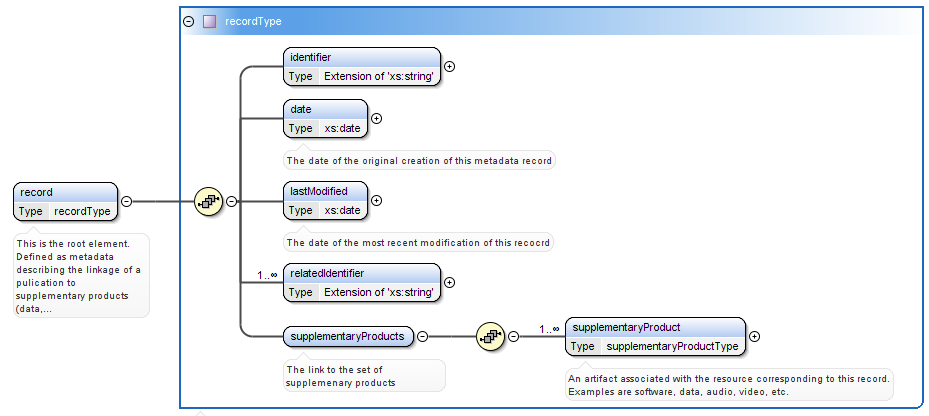
\includegraphics[width=\textwidth]{images/Selection_447.png}
	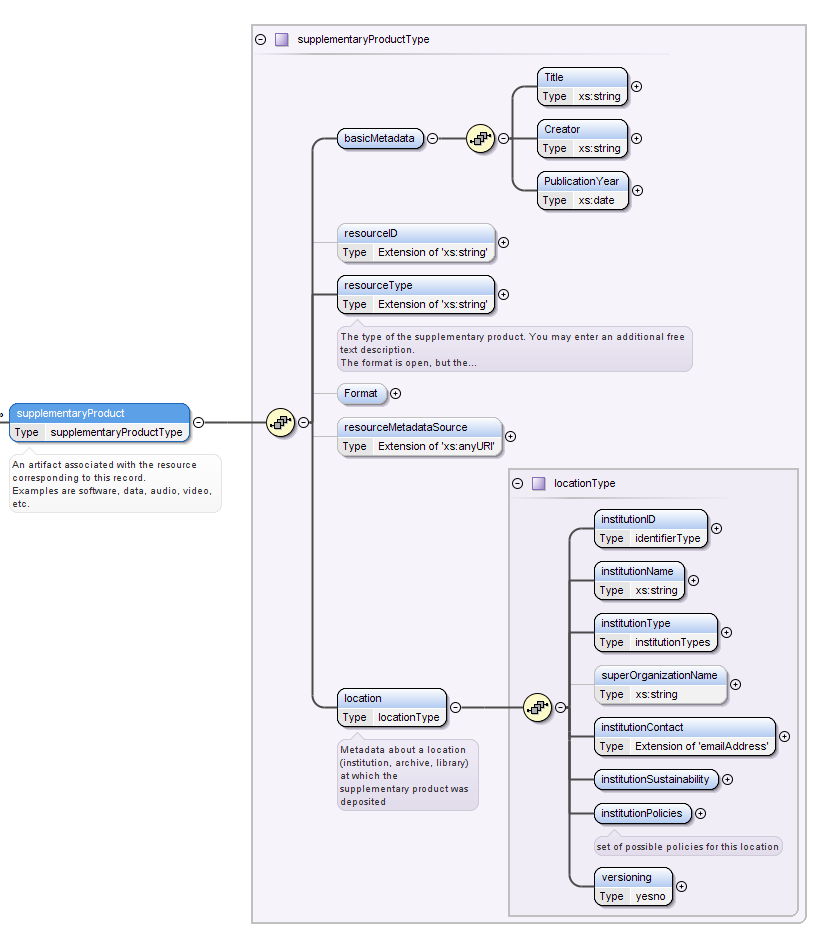
\includegraphics[width=\textwidth]{images/Selection_448.png}
	\caption{\label{fig:schema_v1}High-level structure of proposed package}
\end{figure} 
As shown, each package is structured as a record, which conceptually models a linkage between a publication and its supplementary materials.  As shown, a record has an identity (\ac{DOI}), a date created, a last modified date, and the identity (\ac{DOI}) of the research objects (papers) that are associated with the supplementary products.
Each record then can describe an unlimited number of \texttt{supplementaryProducts}.  Each product has an identifier, a description of its type, licensing information, and linkages to full metadata available elsewhere that fully describes the product.  Each \texttt{supplementaryProduct} has an associated location block, which contains information about the institutional archive at which the respective \texttt{supplementaryProduct} is located.  Finally, for each institution, the set of possible policies are listed, with a boolean designation of the applicability of a policy to the respective supplementary object.   
The full annotated schema is available for examination online at 
\iftoggle{blind}{[URL blinded - please contact JOURNAL]}{\href{https://github.com/labordynamicsinstitute/metajelo}{github.com/labordynamicsinstitute/metajelo}}.

%id;field;description;comment;source;larscomment
\csvreader[/csv/separator=semicolon,/csv/head=true,%
/csv/before reading=\footnotesize%
\setlength{\tabcolsep}{2.5pt},%
/csv/after reading=\normalsize,%
/csv/head to column names=true,%
/csv/longtable=L{0.119\textwidth}L{0.29\textwidth}L{0.3\textwidth}L{0.17\textwidth}L{0.09\textwidth},
/csv/table head=%
 \multicolumn{5}{c}{Table~\thetable : \metajelo Description\label{tab:desc:metajelo}}\\%
 \hline \bf ID & \bf Field &\bf Definition & \bf Notes &\\\hline\endfirsthead%
 \multicolumn{5}{c}{Table~\ref{tab:desc:metajelo} : \metajelo Description}\\%
 \hline \bf ID & \bf Field &\bf Definition & \bf Notes &\\\hline\endhead%
  \hline\endlastfoot%
 \hline&&&\multicolumn{2}{r}{(cont)}\\\endfoot,
/csv/late after line=\\\hline,
table foot=\hline%
]%
{../schema/tabular-metajelo.csv}{}{%
	\id &\texttt{\field} &\description &  \comment & \source 
}

We highlight a few key elements. First, much of the information about the object itself mirrors the DataCite schema \parencite{DataCiteMetadataWorkingGroupDataCiteMetadataSchema2017,DataCiteMetadataWorkingGroupDataCiteMetadataSchema2017a}, even if no \ac{DOI} exists. The bibliographic metadata schema is based on DataCite for simplicity, and is always required. Much of the information on the institution, including its policies, mirrors the re3data schema \parencite{Re3data.Orgre3dataorgMetadata2015,RucknagelMetadataSchemaDescription2015}, with much simplification. In particular, we are interested primarily in \texttt{policyType="Preservation Policy"} and \texttt{policyType="Terms of Use"}. In contrast with the re3data schema, we have merged licenses into the same repeatable element, so that \texttt{policyType="License"} is a valid option. In all cases, we also allow for verbatim capture of the text of the policy, since policies posted on websites, and not versioned, may change over time. We envision either manual entry by the researcher, or webscraping of the provided policy {URL} to populate this field.